\chapter{Basic Fluid Equations and Plasma Flow in Magnetic Nozzle} \label{chap:fluid-equations}
In this chapter, we are going to state the governing equations for the plasma flow in magnetic nozzle. To do this we first start with kinetic description of plasma. By examining the single particle motion along the magnetic field, we make a very important observation, that is magnetic field lines guide the motion of charged particles in plasma. Subsequently we discuss the kinetic description of plasma. Following this, we derive the fluid description of plasma from the kinetic description. The fact that fluid velocity follows the magnetic field line $\mathbf{v} = v\mathbf{B}/B$ will be used to simplify the equations. After this, we establish the governing equations for flow in the magnetic nozzle.

\section{Kinetic Theory}
\subsection{Single Particle Motion in Uniform Magnetic and Electric Fields} \label{sec:single-particle-motion}
Plasma consists of charged particles, and is governed by electromagnetic force. This subsection gives a description of single particle motion with the presence of uniform magnetic and electric fields. This gives us intuition of how the particles move in a magnetic nozzle. Since the particle motion is governed by Lorentz force, the equation of motion of a charged particle is given by
\begin{equation}
	m\dv{\mathbf{v}_p}{t} = q(\mathbf{E} + \mathbf{v}_p\times \mathbf{B}),
	\label{eq:equation-of-motion-single-particle}
\end{equation}
where $m$ is the mass of charged particle, $q$ is its electric charge, and $\mathbf{v}_p$ is the particle's velocity.

\subsubsection*{No Electric Field}
Consider a uniform magnetic field pointing in z-direction, $\mathbf{B}=B\mathbf{\hat{z}}$, and no electric field for now. Since the magnetic force is perpendicular to both $\mathbf{v}_p$ and $\mathbf{B}$, we can separate the equation of motion into two directions,
\begin{equation}
	\begin{aligned}
		m\dv{\mathbf{v_\parallel}}{t} & = \mathbf{0}                  \\
		m\dv{\mathbf{v_\perp}}{t}     & = q\mathbf{v_\perp \times B},
	\end{aligned}
\end{equation}
where $\mathbf{v_\parallel}$ denotes the velocity along the magnetic field line, in this case $v_\parallel = v_z$, and $\mathbf{v_\perp}$ is the velocity perpendicular to the magnetic field, in this case $\mathbf{v_\perp} = v_x\hat{x} + v_y\hat{y}$. Solving these equations with initial condition $\mathbf{v_p}|_{t=0} = v_{0x}\hat{x} + v_{0y}\hat{y} + v_{0z}\hat{z}$ we get
\begin{equation}
	\begin{aligned}
		v_x & = v_{0\perp} e^{i\omega_c t}      \\
		v_y & = \pm iv_{0\perp} e^{i\omega_c t} \\
		v_z & = v_{0z},
	\end{aligned}
\end{equation}
where $v_{0\perp} = \sqrt{v_{0x}^2+v_{0y}^2}$ is the initial speed in the plane perpendicular to the magnetic field, and $\omega_c \equiv \abs{q}B/m$ is called the Larmor frequency. In this way, we see that the charged particle is doing circular motion in the $x-y$ plane with Larmor frequency $\omega_c$. On the other hand, the particle is flowing freely in $\hat{z}$ direction since there is no force acting on the charged particle along the magnetic field line. The charged particle is doing helical motion along the magnetic field line as shown in Fig.~\ref{fig:gyrate-along-b-field}. If we integrate the velocities with respect to time we will see the radius of the gyration is a constant, $r_L \equiv mv_\perp/\abs{q}B$, it is called Larmor radius.

\begin{figure}[htbp]
	\centering
	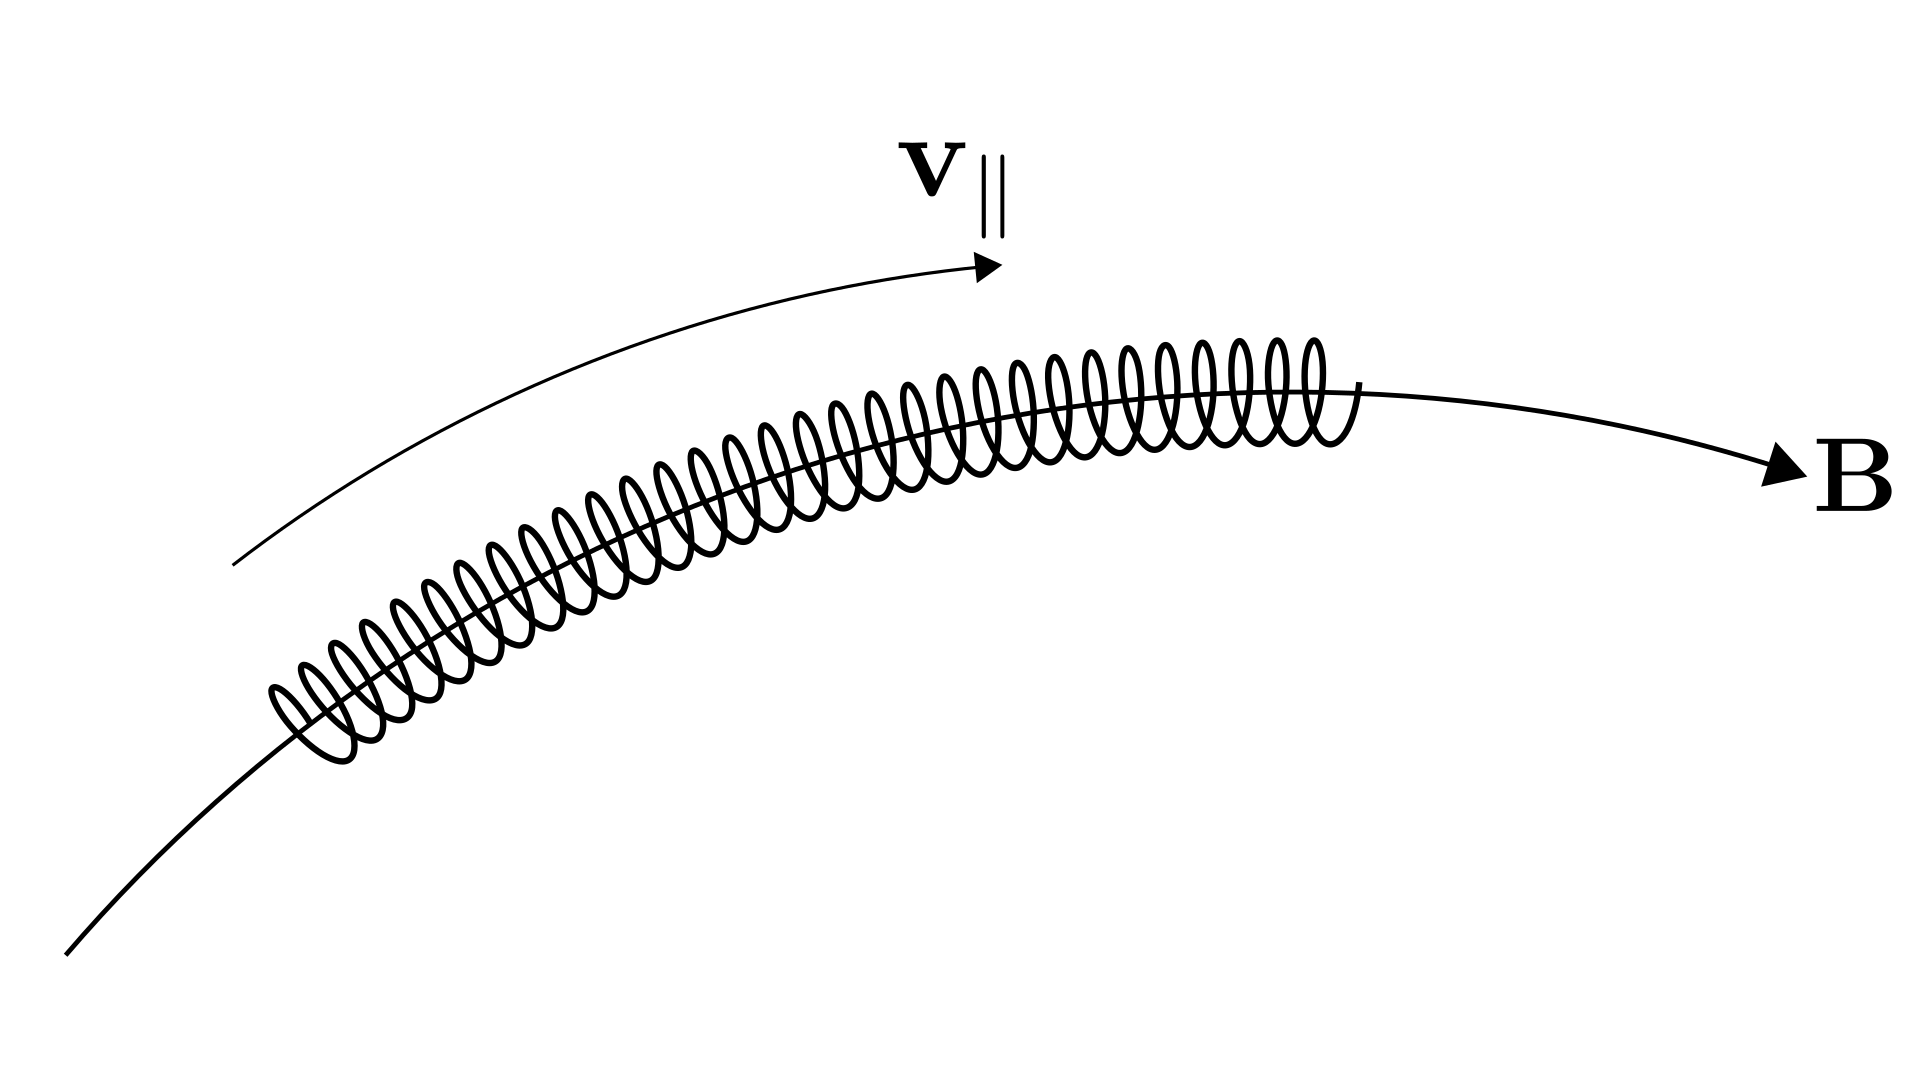
\includegraphics[width=0.7\linewidth]{figures/gyrate-along-b-field}
	\caption{A charged particle gyrates about the magnetic field line. The velocity along the field line is $\mathbf{v}_{\parallel}$ and the Larmor frequency is $\omega_c = \abs{q}B/m$, and the Larmor radius is $r_L = mv_\perp/\abs{q}B$. Moreover, for static, nonuniform magnetic field, the charged particle will stay on the same magnetic field line as it gyrates.}
	\label{fig:gyrate-along-b-field}
\end{figure}


\subsubsection*{Finite Electric Field}
With the presence of uniform electric field $\mathbf{E} = E_x\hat{x} + E_y\hat{y} + E_z\hat{z}$, the solution to Eq.~(\ref{eq:equation-of-motion-single-particle}) becomes

\begin{equation}
	\begin{aligned}
		v_x & = v_{0\perp} e^{i\omega_c t} + \frac{E_y}{B}      \\
		v_y & = \pm iv_{0\perp} e^{i\omega_c t} - \frac{E_x}{B} \\
		v_z & = v_{0z} + \frac{qE_z}{m}t.
	\end{aligned}
\end{equation}
In the direction along the magnetic field, electrostatic force is acting on the particle causing it to accelerate / decelerate with constant acceleration $qE_z/m$. In the direction perpendicular to magnetic field, the Larmor radius is still $r_L = m_v\perp/\abs{q}B$ but the particle's guiding center drifts with velocity
\begin{equation}
	\mathbf{v_{E\times B}} = \frac{\mathbf{E\times B}}{B^2} = \frac{E_y}{B}\hat{x} - \frac{E_x}{B}\hat{y}.
\end{equation}
This is so-called the $\mathbf{E\times B}$ drift.

Imagine a cylinder shape magnetic nozzle with externally applied magnetic field, the magnetic field is as described in Sec.~\ref{sec:magnetic-field-in-nozzle}. The particles will move along the magnetic field lines. Due to high mobility of electrons, they move faster than ions, this creates electric field and will accelerate ions in the nozzle (more details will be discussed in Sec.~\ref{sec:equation-of-motion-of-the-plasma-flow-in-nozzle}). By symmetry, if there is electric field in the plane perpendicular to $\mathbf{B}$ field, it will be pointing radially, $\mathbf{E_\perp} = E_\perp\cos\theta\hat{x} + E_\perp\sin\theta\hat{y}$. According to the above discussion, the $\mathbf{E\times B}$ drift, $\mathbf{v_{E\times B}} = E_\perp/B (\sin\theta\hat{x} - \cos\theta\hat{y})$, will be in $\hat{\theta}$ direction. Meaning that in magnetic nozzle, the particles have two gyrating motions: one is the small scale Larmor gyration, and the other one is the larger scale $\mathbf{E\times B}$ drift in $\hat{\theta}$ direction. In this thesis, we are interested in the flow near the central axis, therefore the larger scale drift will be ignored.

\subsection{Adiabatic Invariant - Magnetic Moment}
For completeness, we introduce the so-called magnetic moment, an adiabatic invariants. We will show that most particles will be trapped in magnetic mirror.

In classical mechanics, the action integral $\oint pdq$ taken over a period of a periodic motion is a constant. Here $p$ and $q$ are generalized momentum and coordinate. In single particle motion along magnetic field line, one obvious periodic motion is the Larmor gyration. Take $p$ to be the angular momentum $mv_\perp r$ and $q$ to be the angular coordinate $\theta$, the action integral becomes

\begin{equation}
	\oint pdq = \oint mv_\perp r_L d\theta = 2\pi r_L mv_\perp = 2\pi \frac{mv_\perp^2}{\omega_c} = 4\pi\frac{m}{\abs{q}}\left(\frac{mv_\perp^2}{2B}\right).
\end{equation}

The magnetic moment is defined as \cite{chen_introduction_2016},
\begin{equation}
	\mu = \frac{mv_\perp^2}{2B}.
\end{equation}

We see that the magnetic moment $\mu$ is constant. If a particle is moving in a magnetic mirror, then due to conservation of magnetic moment (and energy), particles will be reflected at points where magnetic field strength is large. These locations are called turning points and is shown in Fig.~\ref{fig:magnetic-mirror}. Thus only a portion of particles can escape from the magnetic mirror. To be more specific, only particles traveling in the loss cone of the magnetic mirror can pass through, the pitch angle of the loss cone was defined by Eq.~(\ref{eq:loss-cone}).

\begin{figure}[htbp]
	\centering
	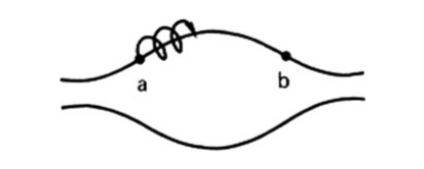
\includegraphics[width=0.7\textwidth]{figures/particle-in-mirror.png}
	\caption{A particle bouncing between turning points $a$ and $b$ in a magnetic mirror. Adapted from \cite{chen_introduction_2016}.}
	\label{fig:magnetic-mirror}
\end{figure}

\subsection{From Kinetic Theory to Fluid Description}
Although the previous treatment is useful for single particle, to describe the collective behavior of a large amount of particles, we need to do that in the framework of kinetic theory. In kinetic theory, the charged particles in plasma obey a certain velocity distribution function,
\begin{equation}
	f(\mathbf{x}, \mathbf{v}_p, t).
\end{equation}
The number of particles per m$^3$ at position $\mathbf{x}$ and time $t$ with velocity components in the cell bounded by $\mathbf{v}$ and $\mathbf{v}+d\mathbf{v}$ is
\begin{equation}
	f(\mathbf{x}, \mathbf{v}_p, t)d^3\mathbf{v}_p.
\end{equation}

Suppose a collisionless plasma in 3-dimensional space is at thermal equilibrium, then the particles can be characterized by Maxwell-Boltzmann distribution,
\[ f_M(\mathbf{x}, \mathbf{v}_p, t) = \frac{n(\mathbf{x}, t)}{(\pi v_{th}^2)^{3/2}} \exp(-\left(\frac{v}{v_{th}}\right)^2), \]
where $n(\mathbf{x},t)$ is number density of the particles, $v_{th} = \sqrt{2k_BT/m}$ is the thermal velocity, and $v=\sqrt{v_x^2+v_y^2+v_z^2}$.

The moments of the distribution function are suitable macroscopic properties of the plasma. For example, the plasma number density and momentum can be viewed as
\begin{equation}
	\begin{aligned}
		n(\mathbf{x}, t)           & = \int_{\mathbb{R}^3} f(\mathbf{x}, \mathbf{v}_p, t) d^3\mathbf{v}_p               \\
		n\mathbf{v}(\mathbf{x}, t) & = \int_{\mathbb{R}^3} \mathbf{v}_p f(\mathbf{x}, \mathbf{v}_p, t) d^3\mathbf{v}_p,
	\end{aligned}
\end{equation}
where $\mathbf{v}$ without the subscript $p$ is the fluid velocity of the plasma flow. It is the bulk velocity of the plasma. The charged particles flow along the magnetic field line, it is intuitive to think of $\mathbf{v}$ as the plasma flow velocity along the magnetic field line.

In this thesis we assume collisionless plasma. The distribution function $f$ in a collisionless plasma satisfies the so-called collisionless Vlasov equation, $\dv*{t} f(\mathbf{x}, \mathbf{v}, t) = 0$. Expand it explicitly, it is
\begin{equation}
	\pdv{f}{t} + \mathbf{v}\pdv{f}{\mathbf{x}} + \frac{q}{m}(\mathbf{E} + \mathbf{v}\times\mathbf{B})\pdv{f}{\mathbf{v}} = 0,
	\label{eq:vlasov}
\end{equation}
where $q(\mathbf{E} + \mathbf{v}\times\mathbf{B})$ is the Lorentz force experience by the species.

Integrate both sides with respect to volume element in velocity space, $d^3\mathbf{v}$, we get the conservation of density.
\begin{equation}
	\pdv{n}{t} + \div(n\mathbf{v}) = 0.
\end{equation}

If we multiply $\mathbf{v}$ on both sides and integrate with respect to $d^3\mathbf{v}$, we get the conservation of momentum,
\begin{equation}
	mn\left[\pdv{\mathbf{v}}{t} + (\mathbf{v}\cdot\grad){\mathbf{v}} \right] = qn(\mathbf{E+v\times B}) - \div\mathbf{P},
\end{equation}
where $\mathbf{P}\equiv mn\overline{\mathbf{v}_{th}\mathbf{v}_{th}}$ is the stress tensor, the bar represents average over velocity space with distribution function $f(\mathbf{x}, \mathbf{v}_p, t)$, is the stress tensor. Here we assume the distribution function is isotropic Maxwellian, then it is easy to see that
\begin{equation}
	\mathbf{P} = \mqty[\dmat[0]{p,p,p}],
\end{equation}
where the isotropic pressure is defined by $p = mn\overline{v_{th,x}^2}$ where $v_{th,x}$ is random thermal velocity in $x$ direction.
\begin{equation}
	mn\left[\pdv{\mathbf{v}}{t} + (\mathbf{v}\cdot\grad){\mathbf{v}} \right] = qn(\mathbf{E+v\times B}) - \grad p
\end{equation}

As we can see the fluid description only depends on the macroscopic properties of plasma, such as the fluid velocity along the magnetic field line $\mathbf{v}$, number density $n$, and pressure $p$ of the plasma. This simplifies the problem.

\section{Equation of Motion of the Plasma Flow in Nozzle} \label{sec:equation-of-motion-of-the-plasma-flow-in-nozzle}
In this section, we will derive the governing equations of the quasineutral plasma flow with cold magnetic ions in magnetic nozzle under paraxial approximation.

Starting from the conservation of number density,
\begin{equation}
	\pdv{n}{t} + \div(n\mathbf{v}) = 0.
\end{equation}
Since ions carry most of the mass and momentum in the plasma, their velocity is more representative of the bulk flow of the plasma. Electrons, on the other hand, have much smaller mass and are highly mobile due to their low inertia, but they contribute less to the overall momentum of the flow. As we discussed in the Sec.~\ref{sec:single-particle-motion}, the charged particles are doing helical motions along the magnetic field lines. Hence, we take the fluid velocity as the ion velocity along the magnetic field lines
\begin{equation}
	\mathbf{v} = v\mathbf{B}/B.
\end{equation}
By expanding the divergence term $\div(n\mathbf{v})$, and using the divergence free condition $\div B=0$, we have
\begin{equation}
	\pdv{n}{t} + \mathbf{B}\cdot \grad(\frac{nv}{B}) = 0.
\end{equation}
Using the paraxial approximation, $\grad_\parallel = \partial_z\hat{z}$. We obtain the conservation of density for the magnetic nozzle,
\begin{equation}
	\pdv{n}{t} + B\pdv{z}(\frac{nv}{B}) = 0.
\end{equation}

The conservation of momentum for ions and electrons are
\begin{align}
	 & m_in\left[\pdv{\mathbf{v}}{t} + (\mathbf{v}\cdot\grad)\mathbf{v}\right] = en(\mathbf{E}+\mathbf{v}\times\mathbf{B})                 \\
	 & m_en\left[\pdv{\mathbf{v}}{t} + (\mathbf{v}\cdot\grad)\mathbf{v}\right]  = -en(\mathbf{E}+\mathbf{v}\times\mathbf{B}) - \grad{p_e},
\end{align}
where $p_e$ is the electron pressure, and cold ions were assumed. There are some simplifications, first is that the term $\mathbf{v\times B} = 0$ due to the fact that fluid velocity is along $\mathbf{B}$. Secondly, $m_en\dv{\mathbf{v}}{t} \simeq 0$ due to small electron mass. Hence, the above two equations becomes,
\begin{align}
	 & m_in\left[\pdv{v}{t} + v\pdv{v}{z}\right] = enE_\parallel \\
	 & 0 = -enE_\parallel - \pdv{p_e}{z}.
\end{align}
Adding these two equations we obtain
\begin{equation}
	\pdv{v}{t} + v\pdv{v}{z} = -\frac{1}{m_in}\pdv{p_e}{z}.
\end{equation}

Assume isothermal, then the electron pressure, also called the equation of state, is
\begin{equation}
	p_e = nKT_e.
	\label{eq:eos}
\end{equation}
We can make this assumption due to the fact the electrons are so mobile that their heat conductivity is almost infinite \cite{chen_introduction_2016}.

Therefore, we have
\begin{equation}
	\pdv{v}{t} + v\pdv{v}{z} = -c_s^2\frac{1}{n}\pdv{n}{z},
\end{equation}
where $c_s^2 = KT_e/m_i$ is the square of ion sound speed. Since we assumed isothermal electrons, so ion sound speed is a global constant.

Therefore, the dynamics of the plasma flow in magnetic nozzle can be characterized by the conservation of density and momentum,
\begin{align*}
	 & \pdv{n}{t} + B\pdv{z}(\frac{nv}{B}) = 0                 \\
	 & \pdv{v}{t} + v\pdv{v}{z} = -c_s^2\frac{1}{n}\pdv{n}{z}.
\end{align*}
The magnetic field profile was discussed in Sec.\ref{sec:magnetic-field-in-nozzle}.

From the above derivation, it is clear that due to finite temperature and high mobility of the electrons, they establish the electric field to accelerate the cold magnetized ions in the nozzle. The thermal energy of the electrons are converted to kinetic energy of ions in this setup.

For convenience, we nondimensionalize the governing equations by normalizing the velocity to $c_s$; i.e., $v\mapsto v/c_s$. The unit of velocity can be written 1 or Mach. $z$ to system length $L$, $z \mapsto z/L$ and time $t\mapsto c_s t/L$. The governing equations become
\begin{align}
	 & \pdv{n}{t} + n\pdv{v}{z} + v\pdv{n}{z} - nv\frac{\partial_z B}{B} = 0
	\label{eq:conservation-of-density}
	\\
	 & n\pdv{v}{t} + nv\pdv{v}{z} = -\pdv{n}{z}.
	\label{eq:conservation-of-momentum}
\end{align}
In the later thesis, we will refer the governing equations to Eq.~(\ref{eq:conservation-of-density}), (\ref{eq:conservation-of-momentum}) without mentioning the nondimensionalization.

\section{Plasma Flow in the Equilibrium} \label{sec:velocity-profiles}
In this research, we are interested in the stability of such plasma flow in the nozzle at equilibrium. Hence, in this section we will derive the velocity profile of plasma flow in steady state.
\subsection{Velocity Profiles}
Let's denote $n_0$ and $v_0$ as equilibrium density and equilibrium velocity, respectively. Since they are stationary (time independent) solutions to the governing equations Eq.~(\ref{eq:conservation-of-density}), (\ref{eq:conservation-of-momentum}), they satisfy the so-called equilibrium condition (nondimensionalized),
\begin{align}
	 & \pdv{z}(\frac{n_0v_0}{B}) = 0 \label{eq:equilibrium-conservation-of-density}                  \\
	 & v_0\pdv{v_0}{z} = -\frac{1}{n_0}\pdv{n_0}{z} \label{eq:equilibrium-conservation-of-momentum}.
\end{align}

In this section we will solve the equilibrium velocity profile, $v_0$, from the nondimensionalized equilibrium condition, Eq.~(\ref{eq:equilibrium-conservation-of-density}) and Eq.~(\ref{eq:equilibrium-conservation-of-momentum}).
We start by substituting $\frac{1}{n_0}\pdv*{n_0}{z}$ into Eq.~(\ref{eq:equilibrium-conservation-of-density}), then it becomes
\begin{equation}
	(v_0^2-1)\pdv{v_0}{z} = -\frac{v_0}{B}\pdv{B}{z}.
\end{equation}

Notice that there is a singularity at $v_0=1$, the sonic speed. Later we will devote an entire Chap.~\ref{chap:singular-perturbation} to discuss the treatment for solving eigenvalues involving this singularity.

We can solve the equation by separating the variables, i.e. $v_0$ on one side and $B$ on the other side of the equal sign. Then integrate equation with respect to $z$ and use the conditions at midpoint $B(0)=B_m, v_0(0)=v_m$ we get
\begin{equation}
	v_0^2e^{-v_0^2} = \frac{B^2}{B_m^2}v_m^2e^{-v_m^2}.
\end{equation}

In order to express $v_0$ as a function spatial coordinate $z$, we introduce a special function called Lambert W function.

\begin{definition}
	The Lambert W function is a function, $W(x)$, such that $ye^y = x$ holds, where $x,y\in\mathbb{R}$.
\end{definition}
Lambert W function has two real branches, $W_0(x)$ the principal branch and the branch $W_{-1}(x)$. They are drawn on Fig.~\ref{fig:lambert-w}. The principal branch is the upper part of relation (blue curve) in the figure, it is defined on $[-1/e, \infty)$ and has range $[-1, \infty)$. The other real branch is the bottom part of the relation (orange curve), and its domain is $[-1/e, 0)$ and range is $(-\infty, -1]$. The point $(-1/e,-1)$ satisfies the equation $ye^y=x$ therefore this point is on the graph of $W(x)$, yet the derivative of $W(x)$ at $-1/e$ is undefined.

\begin{figure}[htbp]
	\centering
	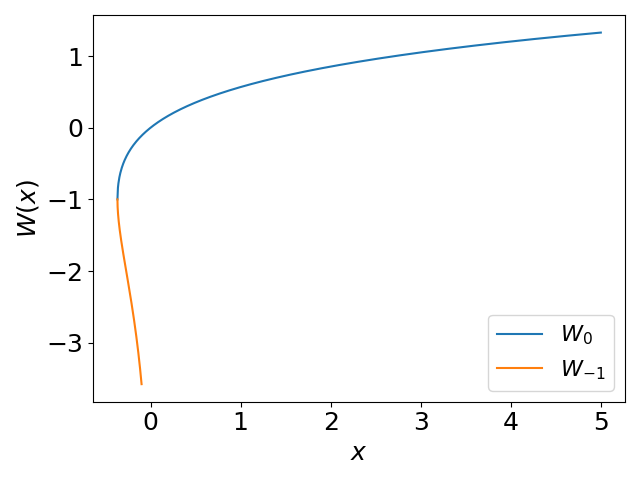
\includegraphics[width=0.6\textwidth]{figures/lambert-w.png}
	\caption{The graph of $y=W(x)$ for real $x<5$ and $y>-4$. The upper branch (blue) with $y\geq-1$ is the graph of the function $W_0(x)$ (principal branch), the lower branch (orange) with $y\leq -1$ is the graph of the function $W_{-1}(x)$. The left most point of the curve is at $(-1/e,-1)$.}
	\label{fig:lambert-w}
\end{figure}

We can now express $v_0$ using the Lambert W function,
\begin{equation}
	v_0(z) = \left[ -W_k\left(-\frac{B(z)^2}{B_m^2}v_m^2e^{-v_m^2}\right) \right]^{1/2},
	\label{eq:velocity-profile}
\end{equation}
where the subscript $k$ of $W$ stands for branch of Lambert W function. Again, the velocity profile is normalized to ion sound speed.

When considering the velocity profile of a nozzle flow, various scenarios can be distinguished based on the Mach number parameter ($v_m$) and the branch ($k$) used in the expression for the Mach number distribution, denoted as $v_0(z)$. These parameters play a crucial role in determining the flow characteristics. The selection of appropriate $v_m$ and $k$ values facilitates the control of the flow characteristics in the nozzle, allowing for the realization of various flow regimes, such as subsonic, supersonic, transonic, accelerating, or decelerating profiles. Different velocity profiles are shown in Fig.~\ref{fig:velocity-profiles}.
\begin{itemize}
	\item Subsonic profile: when $v_m < 1$ and $k = 0$, the resulting velocity profile is classified as subsonic. This means that both at the entrance and exit of the nozzle, the velocity remains subsonic, and the midpoint velocity is also less than unity ($v_m < 1$). A subsonic flow is characterized by fluid velocities that are slower than the local speed of sound. The blue and orange curves on Fig.~\ref{fig:velocity-profiles} are both subsonic profiles. As $z$ goes from $-1$ to $0$, the point $(z,W)$ moves towards the point $(-1/e, 1)$ along the $k=-1$ branch. As $z$ goes from $0$ to $1$, the point $(z, W)$ moves away $(-1/e,1)$ along the same $k=-1$ branch.
	\item Supersonic profile: when $v_m > 1$ and $k = -1$, the velocity profile corresponds to a supersonic flow. In this situation, the fluid velocities at both the entrance and exit of the nozzle are supersonic, and the midpoint velocity ($v_m$) exceeds the value of unity ($v_m > 1$). Supersonic flow is characterized by velocities that surpass the speed of sound. The purple and brown curves on Fig.~\ref{fig:velocity-profiles} are both supersonic profiles. As $z$ goes from $-1$ to $0$, the point $(z,W)$ moves towards the point $(-1/e, 1)$ along the $k=0$ branch. As $z$ goes from $0$ to $1$, the point $(z, W)$ moves away $(-1/e,1)$ along the same $k=0$ branch.
	\item Accelerating profile: when $v_m = 1$, the velocity profile becomes transonic. In this case, the midpoint velocity is exactly at the sonic threshold ($v_m = 1$), where the fluid velocity equals the speed of sound. To achieve an accelerating velocity profile, a configuration with $k = 0$ for $z < 0$ and $k = -1$ for $z > 0$ is employed. Here, $z$ represents the spatial coordinate along the nozzle length. With this setup, the flow starts subsonically and gradually accelerates to a supersonic speed as it propagates along the nozzle. The green curve on Fig.~\ref{fig:velocity-profiles} is the accelerating profile. As $z$ goes from $-1$ to $0$, the point $(z,W)$ moves towards the point $(-1/e, 1)$ along the $k=-1$ branch. As $z$ goes from $0$ to $1$, the point $(z, W)$ moves away $(-1/e,1)$ along another branch, $k=0$.
	\item Decelerating profile: set $v_m = 1$ again, then a decelerating velocity profile can be obtained by adopting a similar approach but with reversed values of $k$. Specifically, the configuration will have $k = -1$ for $z < 0$ and $k = 0$ for $z > 0$, causing the flow to start supersonically and decelerate to subsonic velocities further down the nozzle. The red curve on Fig.~\ref{fig:velocity-profiles} is the decelerating profile. As $z$ goes from $-1$ to $0$, the point $(z,W)$ moves towards the point $(-1/e, 1)$ along the $k=0$ branch. As $z$ goes from $0$ to $1$, the point $(z, W)$ moves away $(-1/e,1)$ along another branch, $k=-1$.
\end{itemize}


\begin{figure}[htbp]
	\centering
	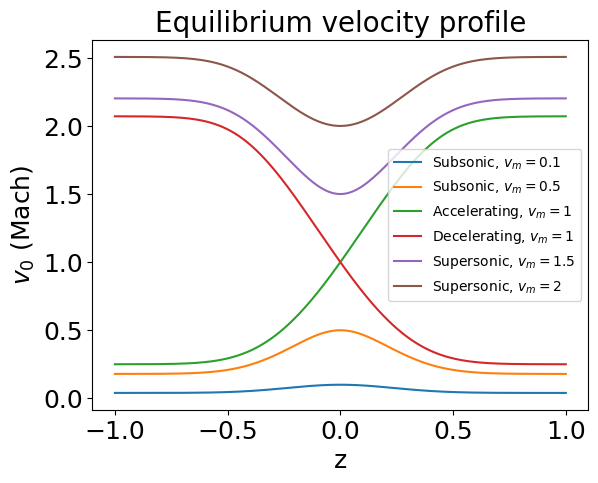
\includegraphics[width=0.7\linewidth]{figures/velocity-profiles}
	\caption{The velocity profile in the magnetic nozzle is completely determined by the midpoint mach number $v_m$ and the branch $k$. A subsonic profile can be obtained by selecting $v_m<1$ and $k=0$. On the other hand, a supersonic profile can be obtained by setting $v_m>1$ and $k=-1$. Lastly, for the transonic velocity profiles, the midpoint velocity is set to unity, $v_m=1$, and then by choose $k=0$ for $x<0$ and $k=-1$ for $x>0$ we get accelerating profile. Decelerating profile can be obtained similarly.}
	\label{fig:velocity-profiles}
\end{figure}
